\documentclass[12pt,letterpaper]{article}
\usepackage[margin=0.62in,headheight=18pt,headsep=18pt,footskip=22pt]{geometry}
\usepackage{tikz}
\usepackage{fancyhdr}
\usepackage[T1]{fontenc}
\usepackage{lmodern}
\usetikzlibrary{arrows.meta}
\pdfinfoomitdate=1
\pdftrailerid{<5745454b38314649534844524146543031><5745454b38314649534844524146543031>}
\pagestyle{fancy}
\fancyhf{}
\fancyhead[L]{\small Week 81 / Buckets of Fish / \band}
\fancyfoot[L]{\scriptsize Bellingham Math Circle / Week 81 / W81-S-draft-v1}
\fancyfoot[R]{\scriptsize\thepage}
\renewcommand{\headrulewidth}{0.3pt}
\renewcommand{\footrulewidth}{0.3pt}
\setlength{\parindent}{0pt}
\setlength{\parskip}{8pt}
\newcommand{\band}{Grades 2--5}
\newcommand{\problem}[2]{\textbf{Problem #1:} #2\par}
\tikzset{fish/.style={circle,fill=black!65,draw=black,minimum size=4.1mm,inner sep=0pt},
 arrow/.style={-{Latex[length=2.3mm]},line width=0.9pt}}
% Miniature diagrams are instructions for setting up the large reusable board.
% All positions and labels read left to right.
\newcommand{\smallstart}[3]{%
\begin{tikzpicture}[x=1cm,y=1cm]
 \foreach \x/\count in {0/#1,1.3/#2,2.6/#3}{
  \draw[rounded corners=2pt,line width=.65pt] (\x,0) rectangle +(1.1,1.15);
  \node[font=\small] at (\x+.55,-.28) {\pgfmathparse{int(\x/1.3+1)}\pgfmathresult};
  \node[font=\large] at (\x+.55,.575) {\count};
 }
\end{tikzpicture}}
\newcommand{\paircard}[2]{%
\begin{tikzpicture}[x=1cm,y=1cm]
 \draw[dashed,black!55] (0,0) rectangle (3.9,2.75);
 \foreach \x/\count/\label in {.45/#1/1,2.15/#2/2}{
  \draw[rounded corners=2pt,line width=.7pt] (\x,.75) rectangle +(1.3,1.25);
  \node[font=\large] at (\x+.65,1.35) {\count};
  \node[font=\small] at (\x+.65,.45) {\label};
 }
\end{tikzpicture}}
\newcommand{\dotsbucket}[4]{% origin x, origin y, count, bucket label
 \draw[rounded corners=2pt] (#1,#2) rectangle +(1.35,1.25);
 \node[font=\scriptsize] at (#1+.675,#2-.22) {#4};
 \foreach \n in {1,...,#3}{
  \ifnum#3>0
   \pgfmathsetmacro{\xx}{mod(\n-1,2)*.43+.44}
   \pgfmathsetmacro{\yy}{floor((\n-1)/2)*.4+.35}
   \node[fish] at (#1+\xx,#2+\yy) {};
  \fi
 }
}
\begin{document}
Take turns. Remove one counter from a nonempty bucket. You may then add counters only to buckets strictly to its left. If you cannot move, you lose.

For Problems 1--3, add at most one counter to each earlier bucket.

\begin{center}
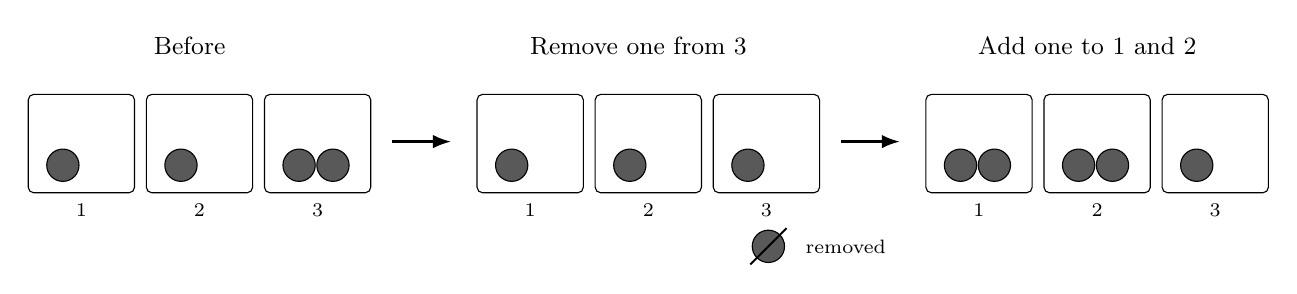
\begin{tikzpicture}[x=1cm,y=1cm]
 \node[font=\small] at (2.05,1.87) {Before};
 \node[font=\small] at (7.75,1.87) {Remove one from 3};
 \node[font=\small] at (13.45,1.87) {Add one to 1 and 2};
 \dotsbucket{0}{0}{1}{1}\dotsbucket{1.5}{0}{1}{2}\dotsbucket{3}{0}{2}{3}
 \dotsbucket{5.7}{0}{1}{1}\dotsbucket{7.2}{0}{1}{2}\dotsbucket{8.7}{0}{1}{3}
 \dotsbucket{11.4}{0}{2}{1}\dotsbucket{12.9}{0}{2}{2}\dotsbucket{14.4}{0}{1}{3}
 \draw[arrow] (4.62,.65)--(5.37,.65);
 \draw[arrow] (10.32,.65)--(11.07,.65);
 \node[fish] at (9.4,-.68) {};
 \draw[black,line width=.75pt] (9.17,-.91)--(9.63,-.45);
 \node[font=\scriptsize,anchor=west] at (9.75,-.68) {removed};
\end{tikzpicture}
\end{center}
\vspace{8pt}
\problem{1}{Play each start with a partner. Which starts let the first player win whatever the second player does?}
\begin{center}
\begin{tabular}{@{}c@{\hspace{.75in}}c@{}}
 \smallstart{0}{0}{1} & \smallstart{1}{1}{0} \\[25pt]
 \smallstart{2}{1}{1} & \smallstart{2}{2}{2}
\end{tabular}
\end{center}
\vspace{12pt}
\begin{tikzpicture}
 \draw[black!35] (0,0) rectangle (17.5,2.5);
\end{tikzpicture}

\newpage
\begin{center}
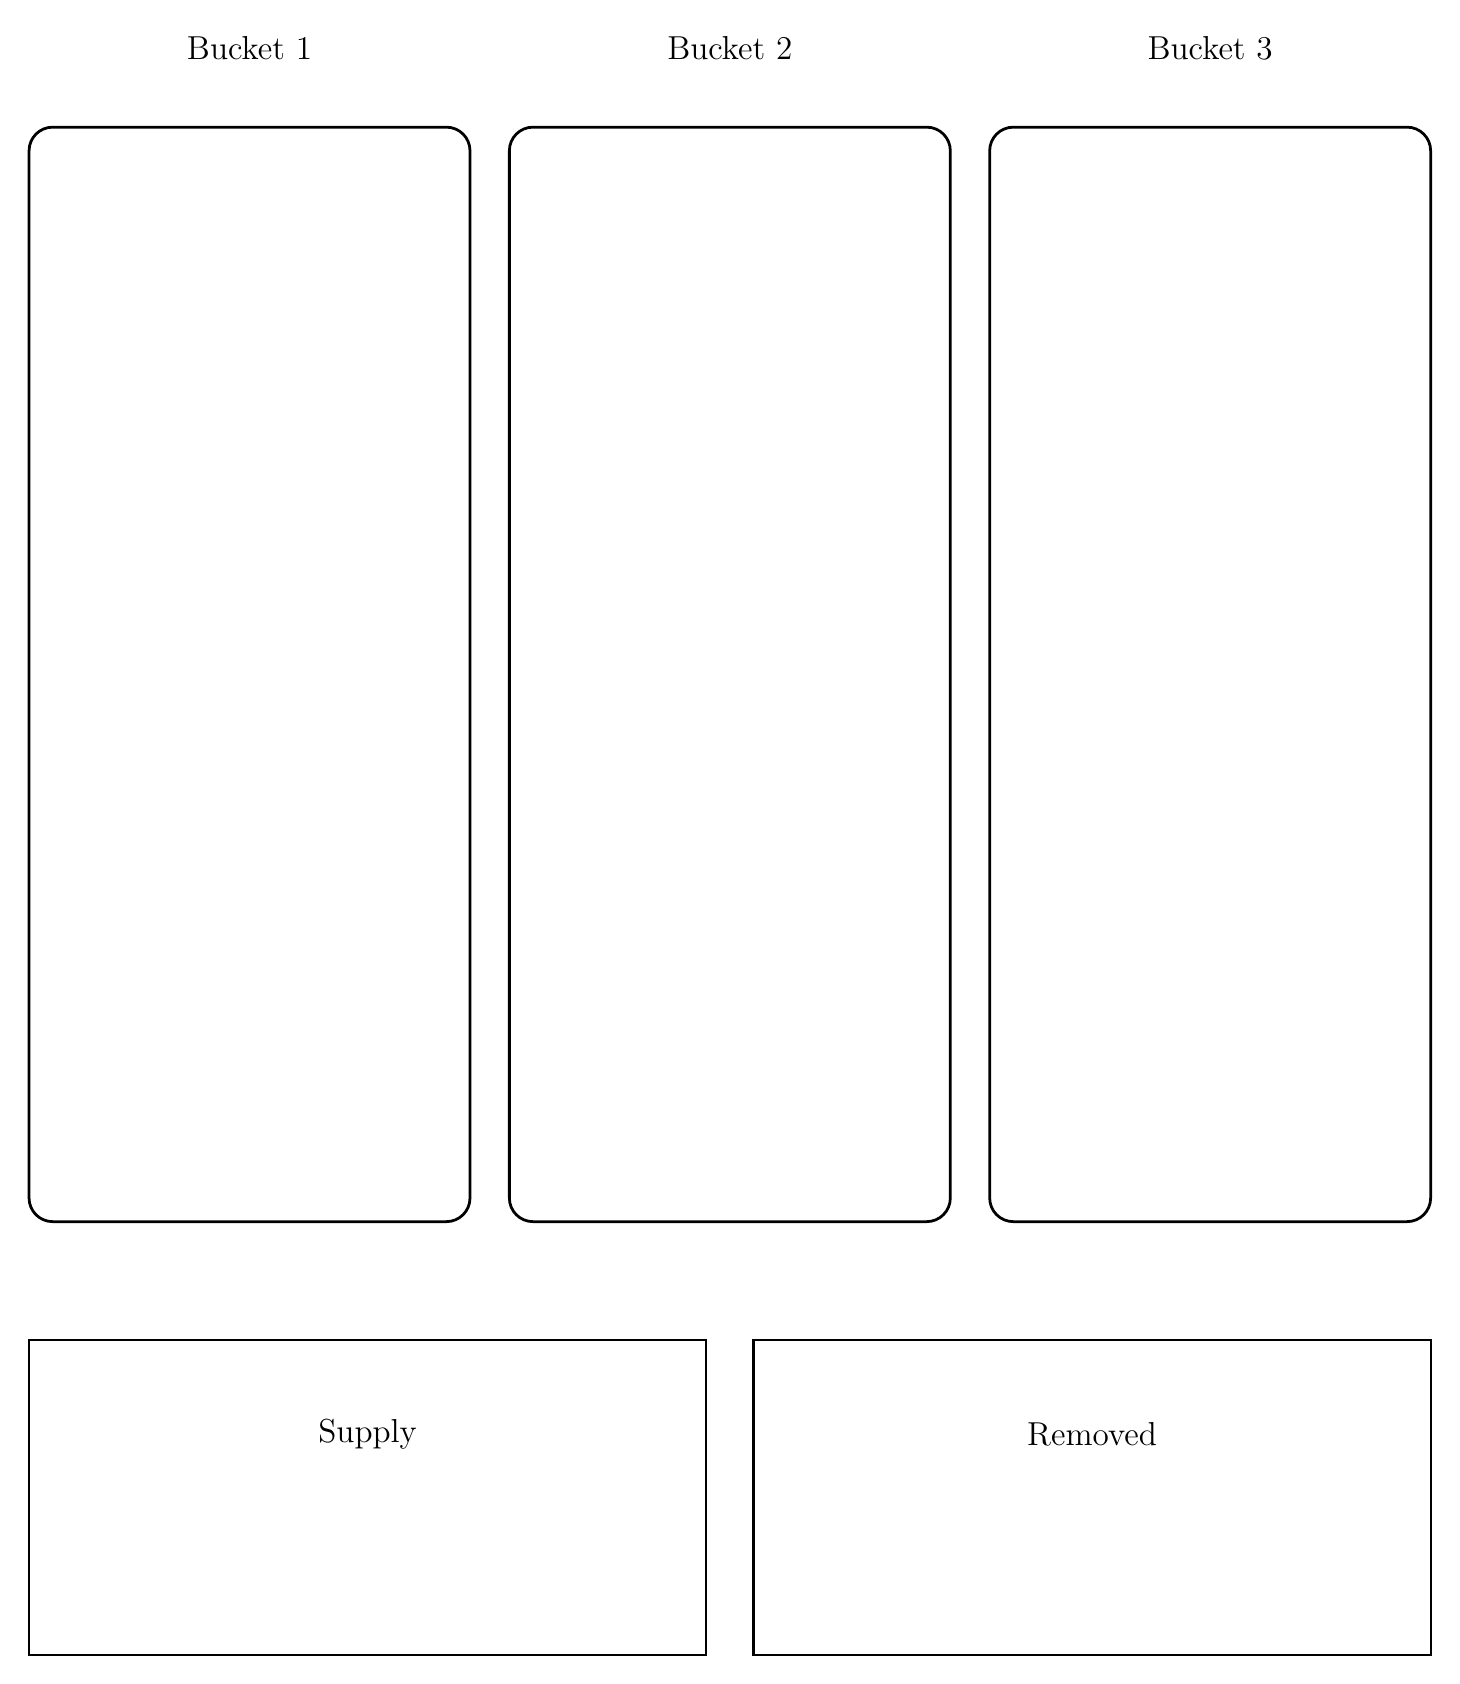
\begin{tikzpicture}[x=1mm,y=1mm]
 \foreach \x/\label in {0/1,61/2,122/3}{
  \node[font=\large] at (28+\x,161) {Bucket \label};
  \draw[rounded corners=3mm,line width=1pt] (\x,12) rectangle +(56,139);
 }
 \draw[line width=.75pt] (0,-43) rectangle (86,-3);
 \draw[line width=.75pt] (92,-43) rectangle (178,-3);
 \node[font=\large] at (43,-15) {Supply};
 \node[font=\large] at (135,-15) {Removed};
\end{tikzpicture}
\end{center}

\newpage
\problem{2}{Use two buckets. Sort these starts into two groups: the first player can force a win, or the second player can force a win.}
\vspace{4pt}
\begin{center}
\begin{tabular}{@{}c@{\hspace{2mm}}c@{\hspace{2mm}}c@{\hspace{2mm}}c@{}}
 \paircard{0}{0}&\paircard{1}{0}&\paircard{2}{0}&\paircard{3}{0}\\[5mm]
 \paircard{0}{1}&\paircard{1}{1}&\paircard{2}{1}&\paircard{3}{1}\\[5mm]
 \paircard{0}{2}&\paircard{1}{2}&\paircard{2}{2}&\paircard{3}{2}\\[5mm]
 \paircard{0}{3}&\paircard{1}{3}&\paircard{2}{3}&\paircard{3}{3}
\end{tabular}
\end{center}

\newpage
\problem{3}{Play from these three-bucket starts. Can you find a rule for choosing a winning move whenever there is one?}
\begin{center}
\begin{tabular}{@{}c@{\hspace{.75in}}c@{}}
 \smallstart{2}{2}{2} & \smallstart{1}{2}{2} \\[22pt]
 \smallstart{2}{1}{2} & \smallstart{2}{2}{1} \\[22pt]
 \smallstart{0}{2}{0} & \smallstart{3}{3}{1}
\end{tabular}
\end{center}
\vspace{10pt}
\begin{tikzpicture}
 \draw[black!35] (0,0) rectangle (17.5,3.8);
\end{tikzpicture}

\newpage
\renewcommand{\band}{Grades 4--5}
For Problems 4--5, a refill may be any finite number of counters. It still goes only to buckets strictly to the left of the bucket you took from.

A number card can stand for that many counters.
\begin{center}
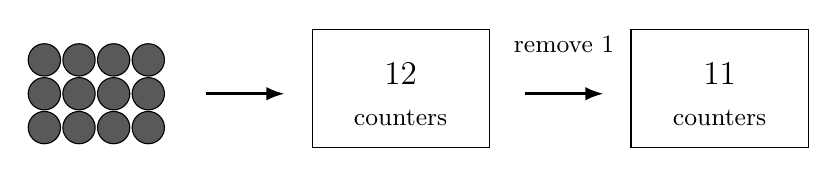
\begin{tikzpicture}[x=1cm,y=1cm]
 \foreach \i in {0,...,11}{
  \pgfmathsetmacro{\xx}{mod(\i,4)*.44}
  \pgfmathsetmacro{\yy}{floor(\i/4)*.43}
  \node[fish] at (\xx,\yy) {};
 }
 \draw[arrow] (2.05,.43)--(3.05,.43);
 \draw (3.4,-.25) rectangle (5.65,1.25);
 \node[font=\large] at (4.525,.68) {12};
 \node[font=\small] at (4.525,.13) {counters};
 \draw[arrow] (6.1,.43)--(7.1,.43);
 \node[font=\small] at (6.6,1.05) {remove 1};
 \draw (7.45,-.25) rectangle (9.7,1.25);
 \node[font=\large] at (8.575,.68) {11};
 \node[font=\small] at (8.575,.13) {counters};
\end{tikzpicture}
\end{center}
\problem{4}{Start with an empty first bucket and one counter in the second. Work together to make a game last at least 10 moves, then 30 moves, then 100 moves. Can you beat any finite number someone names?}
\begin{center}
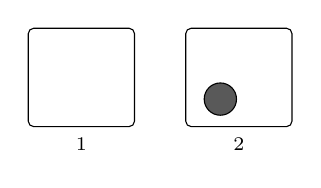
\begin{tikzpicture}[x=1cm,y=1cm]
 \dotsbucket{0}{0}{0}{1}\dotsbucket{2}{0}{1}{2}
\end{tikzpicture}
\end{center}
\vspace{4pt}
\problem{5}{Start with one counter in each of three buckets. Can you agree on moves that keep the game going forever? If you think every game ends, explain why even huge finite refills cannot prevent it.}
\begin{center}\smallstart{1}{1}{1}\end{center}
\vspace{5pt}
\begin{tikzpicture}
 \draw[black!35] (0,0) rectangle (17.5,2.15);
\end{tikzpicture}
\newpage
\begin{center}
\begin{tikzpicture}[x=1mm,y=1mm]
 \foreach \x in {0,61,122}{
  \foreach \y in {0,68}{
   \draw[dashed,black!55] (\x,\y) rectangle +(50,55);
   \draw[line width=.6pt] (\x+7,\y+30)--(\x+43,\y+30);
   \node[font=\large] at (\x+25,\y+17) {counters};
  }
 }
\end{tikzpicture}
\end{center}
\end{document}
